\chapter{Experimental evaluation}
\label{sec:Evaluation}
In order to make the debugging more easier we developed a visualization program. With this program we can draw points or let the program random generate a given number of points. Another function we implemented was to import the given test cases so we can generate our outputs of these curves. This program is very useful especially in the beginning we discovered various errors in our implementation of our algorithm.
We ran a number of test-cases to test our algorithms. The test-cases were generated using our visualization program, which has the ability to draw points on a canvas. This enabled us to easily generate test-cases and test them using the same program. Since the visualization program automatically draws the algorithm's output, errors are easily spotted. (Take, for example, intersections on a closed curve test-case). The program also has a random point generation option.\\
We ran the experiments on a HP Compaq 8510w Laptop with the following specifications:\\
2,4 GHz Intel Core 2 Duo processor T7700\\
2 GB memory.

\begin{center}
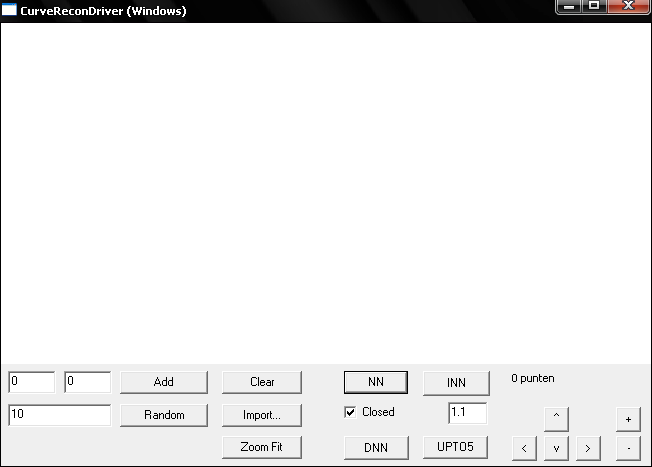
\includegraphics{Evaluation/debugprogram.png}
Figure 9: GUI of visualization program
\end{center}